% !TEX program = xelatex
% 编译: xelatex report.tex （需编译两次以生成页数引用）
\documentclass[a4paper,11pt,fontset=windows]{ctexart}

\usepackage{amsmath,amssymb,bm}
\usepackage{geometry}
\geometry{a4paper, top=2.5cm, bottom=2.5cm, left=2.8cm, right=2.8cm}
\usepackage{graphicx}
\usepackage{booktabs}
\usepackage{array}
\usepackage{enumitem}
\usepackage{xcolor}
\usepackage{caption}
\usepackage{fancyhdr}
\usepackage{lastpage}
\usepackage[hidelinks]{hyperref}

\hypersetup{
  pdftitle={基于神经算子的 Burgers 方程传播前沿预测：公开数据上的泛化与物理修正},
  pdfsubject={Burgers 方程；神经算子；FNO；物理信息机器学习},
  bookmarksnumbered=true
}

\captionsetup{font=small, labelsep=quad}
\captionsetup[figure]{name=图}
\captionsetup[table]{name=表}

\linespread{1.32}
\setlength{\parskip}{2pt}

\ctexset{
  section = {
    format   = \Large\bfseries,
    beforeskip = 16pt,
    afterskip  = 8pt,
  },
  subsection = {
    format   = \large\bfseries,
    beforeskip = 12pt,
    afterskip  = 6pt,
  }
}
\renewcommand{\thesubsection}{\arabic{section}.\arabic{subsection}}

\renewcommand{\topfraction}{0.92}
\renewcommand{\bottomfraction}{0.85}
\renewcommand{\textfraction}{0.08}
\renewcommand{\floatpagefraction}{0.72}

\setlength{\textfloatsep}{16pt plus 3pt minus 3pt}
\setlength{\intextsep}{12pt plus 3pt minus 3pt}
\setlength{\floatsep}{14pt plus 3pt minus 3pt}
\setlength{\abovecaptionskip}{6pt}
\setlength{\belowcaptionskip}{2pt}
% 浮动页：图/表之间不留大块空白，空白推到底部
\makeatletter
\setlength{\@fptop}{0pt plus 1fil}
\setlength{\@fpsep}{14pt plus 2pt minus 2pt}
\setlength{\@fpbot}{0pt plus 1fil}
\makeatother

\pagestyle{fancy}\fancyhf{}
\fancyfoot[C]{\small 第 \thepage 页 / 共 \pageref{LastPage} 页}
\renewcommand{\headrulewidth}{0pt}

\setlist[enumerate]{itemsep=2pt, topsep=4pt, parsep=0pt, leftmargin=2.2em}
\setlist[itemize]{itemsep=2pt, topsep=4pt, parsep=0pt, leftmargin=1.8em}

\begin{document}

\begin{center}
  {\LARGE\bfseries 基于神经算子的 Burgers 方程传播前沿预测：\\[2pt]
   公开数据上的泛化与物理修正\par}
  \vspace{10pt}
  {\small\color{gray} 2026 年 11 月\par}
\end{center}

\vspace{6pt}

\section*{摘要}
\addcontentsline{toc}{section}{摘要}

本文基于 PDEBench 公开的 1D Burgers 数据，研究神经算子对传播激波/前沿的预测能力。以
FNO1D 为主模型、U-Net1D 为基线，先做一步监督训练，再尝试加入 Burgers 方程残差进行微调。
实验表明，FNO1D 的一步相对 $L_2$ 误差为 $1.84\times 10^{-3}$，100 步自回归 rollout 平均误差为
$0.077$，明显优于 U-Net1D 的 $5.79\times 10^{-3}$ 和 $0.433$。一步 PDE 微调把 rollout 平均误差
进一步降到 $0.061$，但三个随机种子的误差棒有重叠，只能视为小幅改善。分布外实验中，模型对更尖锐
的 $\nu=0.001$ 仍能保持较小的前沿速度误差，但对更平滑的 $\nu=0.1$ 基本失效，呈现出明显的不对称性。
sequence-level PDE loss 和多 $\nu$ 参数条件化均未取得正收益，本文将其作为负结果进行分析。

\vspace{4pt}
\noindent\textbf{关键词：Burgers 方程；神经算子；Fourier Neural Operator；物理信息机器学习；分布外泛化}

\section{引言}

Burgers 方程
\begin{equation}
  u_t + u\,u_x = \nu\,u_{xx}
\end{equation}
是流体、交通流和非线性波中的经典 PDE。粘性项会使初始波形形成传播的激波/前沿，因此它既能体现
PDE 结构，又适合作为神经算子代理模型的测试问题。本文使用 PDEBench 公开数据，主要目标围绕这
三个问题展开：

\begin{enumerate}
  \item FNO1D 能否准确预测 Burgers 的时空演化？
  \item 加入 PDE 残差能否改善长时间 rollout？
  \item 从单一 $\nu$ 训练出的模型，能否泛化到更尖锐或更平滑的 $\nu$？
\end{enumerate}

本文的主要工作包括：

\begin{enumerate}
  \item 在 PDEBench 1D Burgers 上建立 FNO1D / U-Net1D 基线；
  \item 比较一步 PDE 残差微调与 data-only 微调；
  \item 构造 $\nu=0.001$ 和 $\nu=0.1$ 的 OOD 测试；
  \item 引入前沿位置/速度指标，分析全局 $L_2$ 之外的行为；
  \item 报告 sequence-level PDE 和多 $\nu$ 条件化的负结果。
\end{enumerate}

\section{数据}

数据来自 PDEBench 的 \texttt{1D\_Burgers\_Sols\_Nu0.01.hdf5}（DOI: 10.18419/darus-2986）。
单个文件约 7.7 GB，直接下载全部数据速度慢，且没有必要。本文的具体处理过程是：先读取 HDF5 中的
\texttt{tensor}、\texttt{t-coordinate} 和 \texttt{x-coordinate}，确认数据形状；再用 HTTP Range
只请求前 200 条轨迹，保存为本地 \texttt{.npz} 文件。PDEBench 的 Burgers 文件里
\texttt{t-coordinate} 有 202 个时间边界，而 \texttt{tensor} 只有 201 个时间快照，因此读取后将时间
坐标截断到 201 个，避免维度不一致。

数据结构：
\begin{equation}
  u \in \mathbb{R}^{200 \times 201 \times 1024}
\end{equation}
三个维度分别为样本、时间和空间；$x\in[0,1]$，$t\in[0,2.01]$。按轨迹划分为 160 条训练、20 条验证、
20 条测试，避免同一轨迹的时空点同时出现在训练集和测试集。归一化统计量只从训练集计算，验证集、
测试集和 OOD 数据都沿用这组均值和标准差，防止信息泄漏。

OOD 数据：
\begin{enumerate}
  \item $\nu=0.001$：100 条轨迹，前沿更尖锐；
  \item $\nu=0.1$：100 条轨迹，前沿更平滑。
\end{enumerate}

OOD 评估取前 20 条轨迹，rollout 100 步。这里有意改变 $\nu$，从而让一个方向让激波更尖锐，另一个
方向让激波更平滑，从而可以用来观察模型在不同前沿尺度上的失效模式。

\begin{quote}
  \small 严格说，Burgers 数据中的结构是粘性激波/传播前沿，不是单一速度的永久行波。本文使用“前沿”一词。
\end{quote}

\section{方法}

\subsection{FNO1D}

FNO1D 由 lifting 层、若干 Fourier block 和 projection 层组成。每个 Fourier block 包含：
\begin{enumerate}
  \item 保留低阶模态的谱卷积；
  \item 逐点卷积；
  \item GELU 激活。
\end{enumerate}

谱卷积只保留前 16 个 Fourier 模态，把其余高频分量置零；每个 block 将谱卷积与逐点卷积分支相加，
再经过 GELU。输入为归一化剖面 $u(t)\in\mathbb{R}^{1024}$，输出为 $u(t+1)$。选择 FNO 的原因是它
通过频域卷积获得全局感受野，更适合描述前沿在空间上的整体传播；U-Net 的感受野主要受卷积核和
下采样层数限制，对长时间、长距离传播的建模能力较弱。

\subsection{U-Net1D}

U-Net1D 作为卷积基线，包含两层下采样、两层上采样和跳连。它与 FNO 使用相同的数据划分、标准化和
训练预算。

\subsection{一步 PDE 微调}

在监督训练之后，加入 Burgers 残差：
\begin{equation}
  \mathcal{L} = \mathcal{L}_{\text{data}} + \lambda\,\mathcal{L}_{\text{PDE}}
\end{equation}
\begin{equation}
  R = \frac{u_{t+1}-u_t}{\Delta t} + u_t\frac{\partial u_t}{\partial x}
      - \nu\frac{\partial^2 u_t}{\partial x^2}
\end{equation}
其中时间导数用前向差分，空间一阶、二阶导数用中心差分；所有导数都在物理尺度的 $u$ 上计算，而不是
在标准化后的 $u$ 上计算。为了让 PDE loss 和数据 loss 量级可比，使用无量纲化：
\begin{equation}
  R_{\text{norm}} = R\cdot\frac{\Delta t}{u_{\text{std}}}
\end{equation}
训练时取 $\lambda=10^{-3}$，从 40 epoch 的 checkpoint 出发，再微调 10 个 epoch，学习率降到 $10^{-4}$。
从而在已有的一步预测器上增加局部物理约束。

\subsection{评价指标}

\begin{enumerate}
  \item 一步相对 $L_2$；
  \item 自回归 rollout 的相对 $L_2$（10/50/100 步）；
  \item 前沿位置误差；
  \item 前沿速度误差。
\end{enumerate}

前沿位置用最大空间梯度定位：
\begin{equation}
  x_f(t) = \arg\max_x \left|\frac{\partial u}{\partial x}\right|
\end{equation}
在周期域上用 64 个网格点的窗口跟踪，速度由 $x_f(t)$ 的线性拟合得到。由于数据中可能有多条激波，
跟踪器偶尔会锁到另一条激波上，导致原始位置误差出现约 0.5 的跳变，因此同时报告“去常数偏移后的
位置误差”（aligned position MAE）。raw 指标反映“有没有跟住同一条激波”，aligned 指标反映“轨迹有
没有整体漂移”，两者结合看比单独看全局 $L_2$ 更接近 PDE 关心的传播行为。

\section{实验设置}

\begin{enumerate}
  \item FNO1D：width 32，modes 16，4 个 Fourier block，72,001 参数；
  \item U-Net1D：base width 16，46,001 参数；
  \item 损失：归一化 MSE；
  \item 优化器：AdamW，学习率 $10^{-3}$；
  \item batch size 32；
  \item 40 个 epoch，早停；
  \item FNO 跑 3 个随机种子，U-Net 跑 1 个种子；
  \item PDE 微调：从对应 seed 的 checkpoint 出发，再训练 10 个 epoch，学习率 $10^{-4}$。
\end{enumerate}

训练采用 one-step teacher forcing：每次从轨迹中取相邻两帧 $(u_t,u_{t+1})$，输入 $u_t$，监督
$u_{t+1}$。验证集只用于选择 checkpoint 和早停，测试集不参与调参。FNO 的三个 seed 使用相同的数据
划分和训练预算，报告均值与标准差；U-Net 只跑一个 seed，作为计算量受限下的对照。

\section{结果与分析}

\subsection{基线}

\begin{table}[!htbp]
  \centering
  \footnotesize
  \setlength{\tabcolsep}{5pt}
  \caption{基线模型的一步与自回归精度（rel $L_2$，括号内为标准差）}
  \label{tab:baseline}
  \begin{tabular}{l r c c c c c}
    \toprule
    模型 & 参数量 & 1 步 & 10 步 & 50 步 & 100 步 & 100 步均值 \\
    \midrule
    FNO1D (3 seeds)   & 72,001 & $\bm{0.00184}$ & $0.029$ & $0.079$ & $0.132$ & $\bm{0.077}$ \\
                      &        & (0.00003) & (0.008) & (0.009) & (0.037) & (0.008) \\
    U-Net1D (1 seed)  & 46,001 & $0.00579$ & $0.079$ & $0.505$ & $0.729$ & $0.433$ \\
    \bottomrule
  \end{tabular}
\end{table}

FNO 的一步误差约为 U-Net 的 $1/3$，100 步 rollout 平均误差约为 U-Net 的 $1/5.6$。FNO 能复现斜向
传播的激波/前沿结构，但尖锐前沿被明显平滑。

这个差距不是单纯的参数量差异。FNO 的谱卷积在频域上做全局混合，能一次性看到整个周期域，因此更
容易学到大尺度前沿的传播方向；U-Net 主要依赖局部卷积，感受野随层数增长有限，在自回归 rollout 中
局部误差会逐步累积。另一方面，FNO 只保留前 16 个模态，相当于对高频做低通滤波，因此原始模型能抓住
大尺度传播、却会把尖锐激波抹平。针对这个“全局结构正确、局部锐度不足”的现象，我们后续进行了 PDE
微调。

\begin{figure}[!htbp]
  \centering
  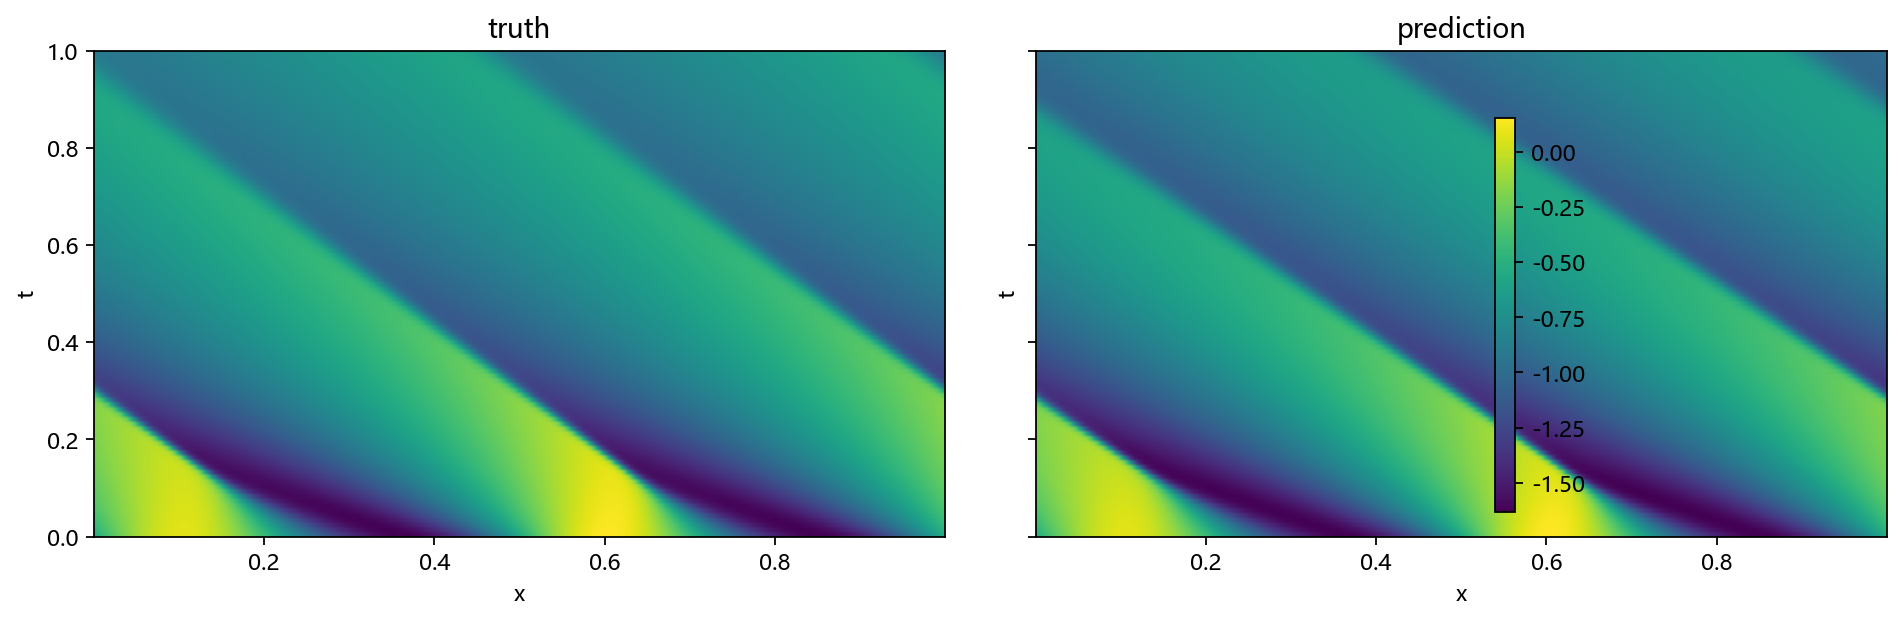
\includegraphics[width=0.92\textwidth]{figures/fno40_rollout_heatmap.png}
  \caption{FNO1D 预测与真值的时空热图（rollout）}
  \label{fig:rollout}
\end{figure}

\begin{figure}[!htbp]
  \centering
  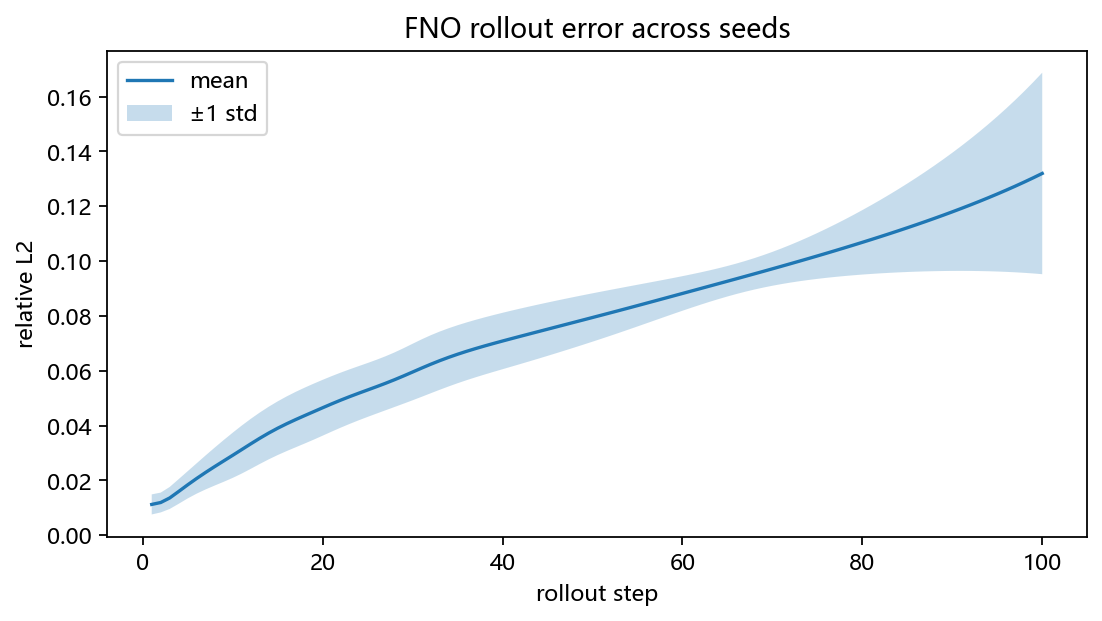
\includegraphics[width=0.68\textwidth]{figures/fno40_rollout_mean_std.png}
  \caption{三个随机种子上的 rollout 误差均值与标准差}
  \label{fig:seed}
\end{figure}

\subsection{一步 PDE 微调}

\begin{table}[!htbp]
  \centering
  \small
  \setlength{\tabcolsep}{8pt}
  \caption{一步 PDE 微调与 data-only 微调的对比}
  \label{tab:finetune}
  \begin{tabular}{l c c}
    \toprule
    模型 & 一步 rel $L_2$ & 100 步平均 \\
    \midrule
    FNO baseline（3 seeds）      & $0.00184\pm0.00003$ & $0.077\pm0.008$ \\
    FNO + data-only FT（3 seeds） & $0.00171\pm0.00021$ & $0.065\pm0.015$ \\
    FNO + PDE FT（3 seeds）      & $\bm{0.00153\pm0.00010}$ & $\bm{0.061\pm0.015}$ \\
    \bottomrule
  \end{tabular}
\end{table}

\begin{figure}[!htbp]
  \centering
  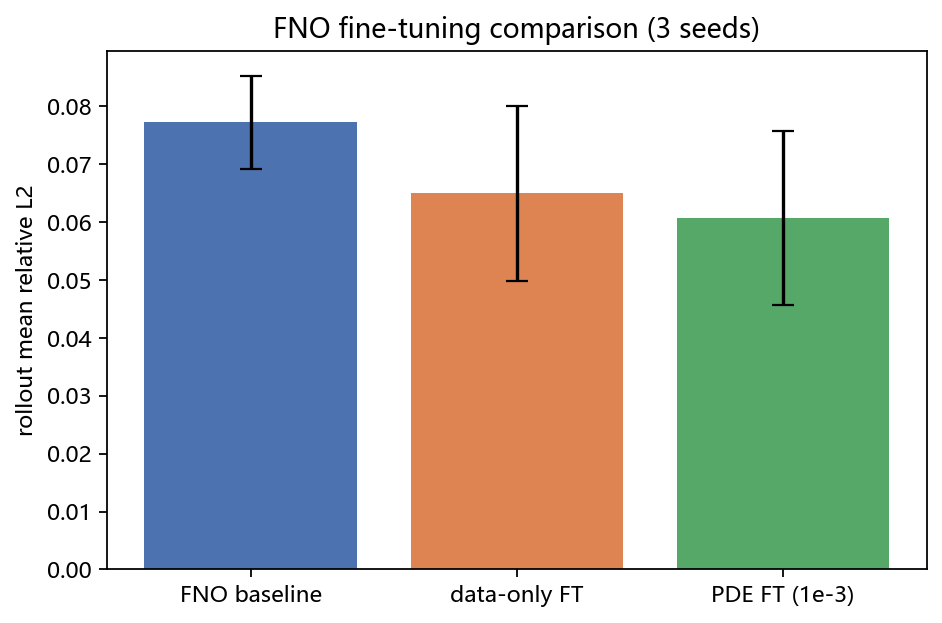
\includegraphics[width=0.72\textwidth]{figures/finetune_rollout_comparison.png}
  \caption{基线、data-only 微调与 PDE 微调的 rollout 误差对比}
  \label{fig:finetune}
\end{figure}

PDE 微调在 one-step 和 rollout 平均上都略有改善，但三个 seed 的误差棒明显重叠，因此只能视为
“有希望”，不能视为统计显著。$\lambda=10^{-2}$ 在 seed 0 上反而变差，说明权重需要调整。

从机制上看，这个结果是可以理解的。当前 PDE 残差只约束 $u_t\to u_{t+1}$ 的局部关系，并没有直接约束
10 步、50 步之后的误差累积；因此它能略微改善一步预测，却不能从根本上解决 rollout 漂移。另外，
data-only 微调本身也会因为多训练了 10 个 epoch 而变好，所以 PDE 的净收益需要用 data-only 作为
对照，不能把“比 40 epoch baseline 好”全部归因于物理损失。

\subsection{OOD 与前沿指标}

\begin{table}[!htbp]
  \centering
  \small
  \setlength{\tabcolsep}{6pt}
  \caption{分布内与分布外（OOD）的前沿指标}
  \label{tab:ood}
  \begin{tabular}{l c c c c}
    \toprule
    模型 & $\nu$ & rollout mean rel $L_2$ & aligned position MAE & speed MAE \\
    \midrule
    FNO baseline & 0.01（ID）    & 0.0765 & 0.0081 & 0.0329 \\
    FNO baseline & 0.001（OOD）  & 0.1591 & 0.0068 & 0.0267 \\
    FNO baseline & 0.1（OOD）    & 0.7897 & 0.0533 & 0.1620 \\
    FNO + PDE    & 0.01（ID）    & $\bm{0.0521}$ & $\bm{0.0052}$ & $\bm{0.0158}$ \\
    FNO + PDE    & 0.001（OOD）  & $\bm{0.1474}$ & $\bm{0.0048}$ & $\bm{0.0180}$ \\
    FNO + PDE    & 0.1（OOD）    & 0.7901 & 0.0524 & 0.1537 \\
    \bottomrule
  \end{tabular}
\end{table}

\begin{figure}[!htbp]
  \centering
  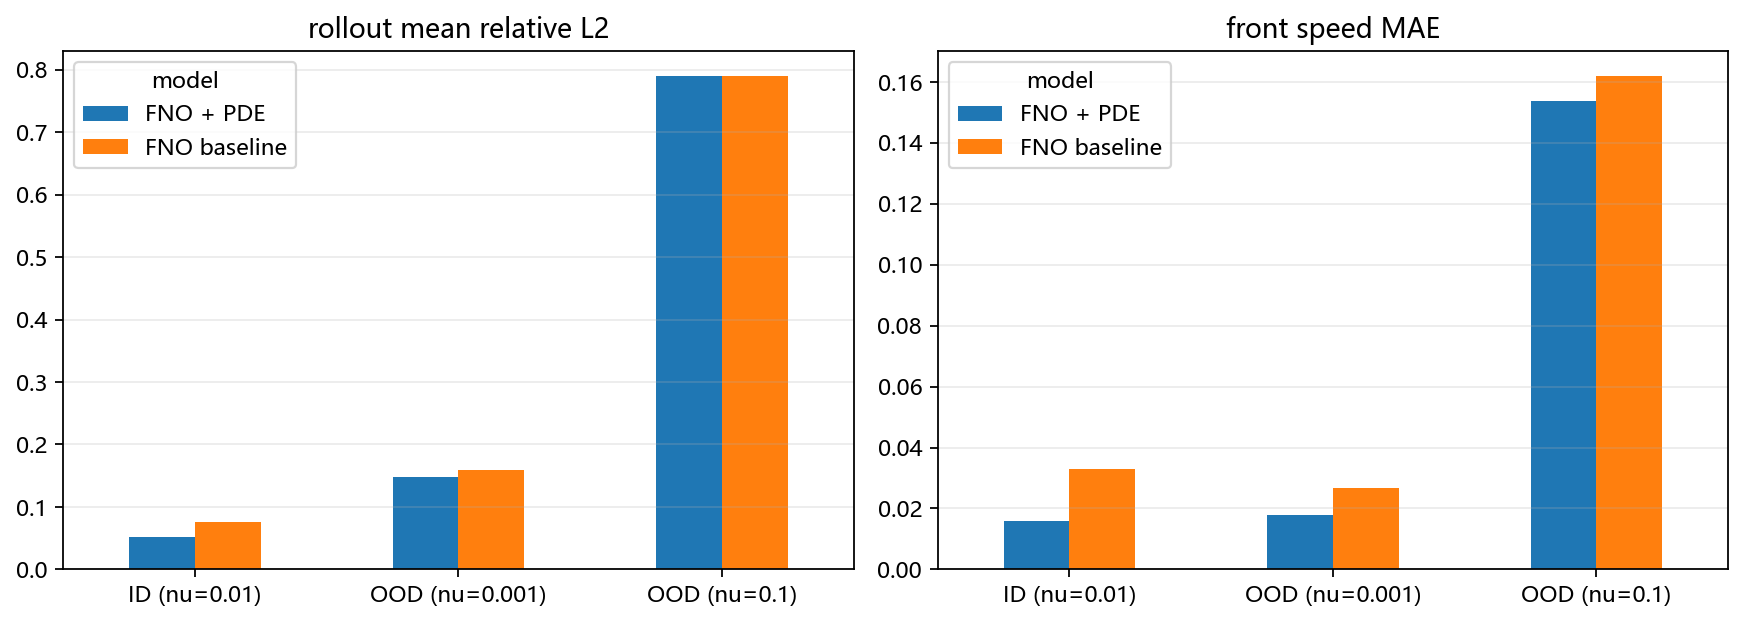
\includegraphics[width=0.95\textwidth]{figures/ood_metrics.png}
  \caption{不同 $\nu$ 下的 rollout 误差与前沿速度误差}
  \label{fig:ood}
\end{figure}

OOD 失败是不对称的：
\begin{enumerate}
  \item 对更尖锐的 $\nu=0.001$，全局 $L_2$ 变差，但前沿位置和速度仍抓得住；
  \item 对更平滑的 $\nu=0.1$，误差接近 0.8，速度误差也很大，模型基本失效；
  \item PDE 微调在 ID 和 $\nu=0.001$ 上略有帮助，但对 $\nu=0.1$ 没有改善。
\end{enumerate}

这种不对称主要是因为“分布差异的大小”。$\nu=0.001$ 的前沿更尖锐，局部梯度更大，但它仍然保留了与
训练集相同的“斜向传播激波”结构；模型虽然画不出最锐的细节，但能抓住前沿的大致位置和速度。相比
之下，$\nu=0.1$ 的粘性明显更强，激波更宽、更平滑，前沿速度和波形结构都偏离训练分布；模型在训练中
从未见过这种平滑 regime，误差就会迅速累积。这说明当前模型学到的更多是 $\nu=0.01$ 附近的特定动力
学，而不是对 Burgers 方程的一般解算子。

\subsection{失败尝试}

Sequence-level PDE loss：把 PDE 残差作用在 $H=5$ 步自回归展开上。PDE 梯度会放大预测
误差，训练不稳定；降低 $\lambda$ 只能部分缓解。$H=2$ 并 detach 第二步后仍无改善，rollout 平均约
0.10，明显差于一步 PDE 微调的 0.061。

多 $\nu$ 联合训练 + 常数 $\log\nu$ 通道：训练 $\nu=0.001/0.01$，留出 $\nu=0.1$。25 epoch
后联合测试 rollout 平均 0.391，留出 $\nu=0.1$ 的 rel $L_2$ 为 8.60，完全失败。说明仅把参数拼成
输入通道不足以解决跨参数泛化。

5.2 和 5.3 作为负结果保留，用于说明“PDE 残差”和“参数条件”并不是无条件有效。sequence PDE 的
核心问题是：自回归展开后的预测误差会进入下一步输入，PDE 残差又把这些带误差的预测纳入梯度，相当
于用不稳定的长轨迹去约束模型；detach 只能切断梯度，不能消除输入分布偏移。多 $\nu$ 条件化的核心
问题则是：常数通道对谱卷积的调制太弱，两个 $\nu$ 的动力学又差异较大，共享的谱卷积很难同时拟合，
最终表现为欠拟合和 OOD 崩溃。

\section{结论}

\begin{enumerate}
  \item 在 PDEBench 1D Burgers 上，FNO1D 的一步和 rollout 精度都明显优于 U-Net1D。
  \item FNO 能捕捉大尺度前沿传播，但会平滑尖锐激波；误差随 rollout 累积。
  \item 一步 PDE 微调带来小幅改善，但方差较大，不能宣称显著优于 data-only。
  \item OOD 泛化是不对称的：更尖锐的 $\nu=0.001$ 相对可接受，更平滑的 $\nu=0.1$ 基本失效。
  \item sequence-level PDE 和多 $\nu$ 常数通道条件化在当前实现下均为负结果。
  \item 当前主结果应使用单 $\nu$ FNO + one-step PDE 微调；跨参数泛化仍未解决。
\end{enumerate}

综上所述，本文最有价值的结论不是“PDE loss 一定有效”，而是在公开 Burgers 数据上，稳定的
one-step 监督训练比复杂的 sequence-level 约束更可靠；轻量 PDE 正则能改善局部精度，但不能替代
长期 rollout 训练；真正的跨 $\nu$ 泛化需要更强的参数条件机制，而不是简单拼接一个常数通道。

\section{局限与复现}

\begin{enumerate}
  \item 只使用 $\nu=0.01$ 的 200 条轨迹作为主训练集，参数覆盖有限；
  \item U-Net 只跑了 1 个 seed，对比不够充分；
  \item PDE 微调只训练 10 个 epoch，权重未系统调优；
  \item 前沿跟踪在有多条激波时可能锁到不同激波，因此同时报告 raw 和 aligned 位置误差。
\end{enumerate}

\begin{thebibliography}{9}
\addcontentsline{toc}{section}{参考文献}
\bibitem{pdebench} Takamoto, M., Praditia, T., Leiteritz, R., MacKinlay, D., Alesiani, F.,
  Pfl\"uger, D., Niepert, M. \emph{PDEBench: An Extensive Benchmark for Scientific Machine
  Learning}. NeurIPS 2022 Datasets and Benchmarks.
\bibitem{fno} Li, Z., Kovachki, N., Azizzadenesheli, K., et al. \emph{Fourier Neural Operator
  for Parametric Partial Differential Equations}. ICLR 2021.
\bibitem{pinn} Raissi, M., Perdikaris, P., Karniadakis, G. E. \emph{Physics-informed neural
  networks: A deep learning framework for solving forward and inverse problems involving
  nonlinear partial differential equations}. Journal of Computational Physics, 2019.
\bibitem{burgers} Burgers, J. M. \emph{A mathematical model illustrating the theory of
  turbulence}. Advances in Applied Mechanics, 1948.
\end{thebibliography}

\end{document}
